\documentclass[aps,preprint]{revtex4-1}
\usepackage{graphicx}
\usepackage{amsmath}
\usepackage{makeidx}
\usepackage{amsfonts}
\usepackage{amssymb}
\usepackage{mathtools}
\usepackage{xcolor}

\begin{document}


\title{Efficiency and entropy production of selfish drivers}



\date{\today}

\begin{abstract}
Characterizing transport processes in a city system is important to have a better picture of efficiency and sustainability in such a complex system. In this study, we consider the process of movements of selfish drivers from their homes (origins) to work places (destinations) to see how interactions and randomness in the movements affect a measure of efficiency and entropy production in this process. Interactions are modelled by the effect of the flows on the local travel times, and by exploiting the travel information from the previous days. Here, the efficiency is computed by comparing the total travel time with the number of travels along the links. And, the entropy production is obtained by comparing the time intervals of leaving the origins and arriving at the destinations. We use  realistic models of population distributions and mobility laws for simulation of the movement process where at each step a driver moves to a neighbouring site which is closer to the destination or which is chosen randomly. We observe that interactions and a naive way of using the travel information without any coordination reduce the efficiency and increase the entropy production of the process. Moreover, the larger systems display smaller efficiencies for the same model parameters like the population density which limits the size of an efficient city. On the other hand, randomness in the movements can help to enhance the efficiency when the strength of interactions is large and congestion is high. We also find that the entropy production is a good order parameter to distinguish the low- and high-congestion phases. In the former phase, the entropy production grows monotonically with the probability of random moves whereas it displays a minimum in the congested phase; that is randomness in the movements can reduce the uncertainty in the destination time intervals. 
\end{abstract}


%\pacs{} 

\maketitle

\section{Introduction}\label{S0}

\begin{itemize}

\item interactions $(g,\lambda)$ increase the travel time, reduce the efficiency, and increase the entropy production.


\item $\lambda=0$: 

- we observe a change in behaviour of the entropy production $\Delta S_D$ vs the disorder parameter $\alpha$ as the interaction strength $g$ increases.  For sufficiently large $g$, a bit of disorder can reduce the entropy production. 


\item $\lambda=0.5$: 

- we observe a change in the complexity of the time series in days as the interaction strength $g$ increases.

- the efficiency and velocity display a (nontrivial) maximum for some disorder $\alpha^*(g)$ depending on the parameter $g$.  

- mutual information between $(t_O,t_D)$ increases whereas that of $(\Delta x_{OD},\Delta t_{OD})$ decreases by introducing $\lambda$. 



\end{itemize}


\section{Models and Settings}\label{S1}
In this section, we present the main definitions and methods which are used to model the network flow dynamics.   
Consider a city of $N$ sites with local populations $\{m_a:a=1,\dots,N\}$ and total population $M=\sum_a m_a$. The connectivity graph of the city is given by $G(V,E)$ where $V$ is the set of sites and $E$ is the set of directed edges $(ab)$. Here we take a two dimensional square lattice of size $N=L\times L$, where all edges have the same length and the same free travel times. We use the simple growth model introduced in Ref. \cite{Li-nc-2017} to produce reasonable population distributions for the model cities. The population density is fixed to $M/N=10^3$ in the following.

Given the population distribution $m_a$, we use the following mobility law to construct the flux of movements $m_{a\to b}$ from origins $a$ to destinations $b$, 
\begin{align}\label{mab}
m_{a\to b}=m_ap_{a\to b}=m_a\frac{m_b/M(r_{ab})}{\sum_{c\neq a} m_c/M(r_{ac})},
\end{align}
where $M(r_{ab})$ is the population in the circle of radius $r_{ab}$ centred at site $b$. The ratio $m_b/M(r_{ab})$ can be interpreted as the attractiveness of site $b$ for an individual at site $a$. 

Finally, the flows of movements on edges $(ab)\in E$ are determined by a flux distribution problem that satisfies the system constraints and preferences, as follows. 
 

\subsection{The movement process}\label{S11}
Here is the process of moving from the origins to destinations in a single day:

\begin{itemize}

\item The starting times of the OD trips are distributed uniformly in the origin time interval $\Delta T_O$. We assume that $\Delta T_O$ is the same for all origins. In each time step, the time increases by $\Delta t=1$. Driver $i$ starts its trip and becomes active at time $t_O(i) \in \Delta T_O$. The trip will become inactive when the driver reaches its destination at time $t_D(i) \in \Delta T_D$. The destination time interval $\Delta T_D$ is determined by the system structure and dynamics (see Fig. \ref{Tday}). 
The arrival times of the drivers to destination site $a$ determine the destination time interval $\Delta T_D(a)$ of that site. 
The travel time from origin to destination for driver $i$ is denoted by $\Delta t_{OD}(i)=t_D(i)-t_O(i)$. 

\item An active driver $i$ at site $a$ chooses the next site as follows: with probability $\alpha$ the next site is chosen randomly and uniformly from the set of neighbouring sites. With probability $1-\alpha$ the neighbour that minimizes the expected travel time to the destination $D(i)$ is selected. The expected travel time on edge $(ab)$ is denoted by $\tilde{t}_{ab}$. The expected travel times in day $d$ are estimated by using the actual travel times $t_{ab}$ from the previous day:
\begin{align}\label{tab0}
\tilde{t}_{ab}(d)=\lambda t_{ab}(d-1)+(1-\lambda) \tilde{t}_{ab}(d-1).
\end{align}
For the initial day $\tilde{t}_{ab}(0)=t_{ab}(0)$, where the $t_{ab}(0)$ are the travel times for free lines. 

\item Let flow $F_{ab}(t)$ be the number of people that enter edge $(ab)$ at time step $t$. Given the input flows, then the actual travel times are obtained from 
\begin{align}\label{tab}
t_{ab}(F_{ab})=t_{ab}(0)\left(1+g(\frac{F_{ab}}{F_{ab}^*})^{\mu}\right),
\end{align}
with $g (F_{ab}/F_{ab}^*)^{\mu}$ to model the influence of flows on the travel times \cite{BPR-1964,lc-trans-1976,lc-trans-2011}. Here $F_{ab}^*$ is a measure of the line capacity. For simplicity, we assume that $t_{ba}(0)=t_{ab}(0)$ and $F_{ba}^*= F_{ab}^*$.
In the following we take $\mu=3$, $t_{ab}(0)=1$, and $F_{ab}^*=M/|E|$ in all simulations.

\end{itemize}

The actual travel time $t_{ab}$ determines the time that a person spends on edge $(ab)$. The total number of persons on edge $(ab)$ at time step $t$ is denoted by the flow density $\rho_{ab}(t)$. 


\section{Results}\label{S2}
Let us start with the effects of interactions on the cumulative distribution of the travel times $P(\Delta t_{OD}>T)$ in the absence of any randomness in the movements ($\alpha=0$). As Fig. \ref{Ti} shows, the travel times increase by introducing the interactions either by considering the effects of flows on the trips (with $g$) or by knowing the travel information from the previous days (with $\lambda$). The latter says that a selfish way of using the information without any coordination could result to a chaotic situation \cite{Apps-ieee-2019}. We know that interacting systems can display complex behaviours and interactions may reduce the system predictability \cite{watts-sci-2006}. In the following, we see how the interplay of the above interactions with disorder in the movements affects a measure of complexity and predictability of the movement process. In addition, we follow the changes in the efficiency and a measure of entropy production in the system to see how the relation between these qualities depend on the macroscopic state (phase) of the system \cite{efc-srep-2020}.  
                    

\subsection{Complexity and predictability}\label{S21}
A measure of predictability for two stochastic variables $x,x'$ is provided by the mutual information of the two variables,
\begin{align}
\mathrm{MI}(x,x')=\sum_{x,x'}P(x,x')\log\frac{P(x,x')}{P(x)P(x')},
\end{align}
where $P(x,x'), P(x)$ and $P(x')$ are the joint and marginalized probability distributions of the variables.

Let us define the mutual information between the destination and origin times
\begin{align}
\Pi_{t,t}=\mathrm{MI}(t_O,t_D),
\end{align}
and the mutual information between the travel time and the geometrical distance, 
\begin{align}
\Pi_{x,t}=\mathrm{MI}(\Delta x_{OD},\Delta t_{OD}).
\end{align}
Figure \ref{Pi} shows the results of numerical simulations for these quantities in a square lattice of linear size $L=20$.
As expected, the above measures of predictability diminish with increasing $g$ or $\alpha$, except the small jump that is observed 
for $\lambda=0.5$ when $\alpha$ changes from zero.  On the other hand, we observe that $\Pi_{t,t}$ increases but $\Pi_{x,t}$ decreases after using the travel times from the previous days (i.e., for $\lambda=0.5$). Note that when $\lambda=0$ all edges have the same estimated travel times $\tilde{t}_{ab}(d)=t_{ab}(0)=1$ where the shortest path is strongly correlated with the geometrical distance $\Delta x_{OD}$. On the other side, when $\lambda=0.5$ there are some edges with small travel times in the previous day and all drivers are aware of this information which in turn determines the shortest path to their destinations. Therefore, one expects to observe less correlations here between the geometrical distance and the actual travel times. However, the same global information now makes the arrival times to the destinations more dependent on the departure times from the origins and results to larger mutual information between the two time variables. 


To address the complexity of the process, we check the presence of long range correlations in the time evolution of the system. 
Consider a stationary time series $\{\cdots,x_{n-1},x_n,x_{n+1},\cdots\}$ and a string of data points which is divided into two equal data sets $\mathbf{x}_{past}$ and $\mathbf{x}_{future}$ of length $l$. A measure of complexity can be defined by the scaling of the mutual information $\mathrm{MI}(\mathbf{x}_{past},\mathbf{x}_{future})$ with $l$. This information could be independent of the size or increase logarithmically or even sub-linearly with $l$ \cite{bialek-nc-2001}. In the following, however, we study a computationally more efficient but approximate way of detecting a time series complexity, which is based on an estimation of information rate (sample entropy) in different time scales \cite{samp-ajp-2000,costa-prl-2002}. 

Consider the coarse grained time series $\{\cdots,y_{n-1},y_n,y_{n+1},\cdots\}$ obtained by averaging the original time series within a window of size $w$, i.e., $y_n=(\sum_{n'=(n-1)w+1}^{nw}x_{n'})/w$. Let $\mathbf{y}_n(l)$ be a sequence of length $l$ starting at $n$. We define $p(l:r,w)$ as the probability that two such sequences are within distance $r$ of each other, i.e., $d(\mathbf{y}_n(l),\mathbf{y}_{n'}(l))<r \times std(x)$. Here $d(\mathbf{y}_{n_1}(l),\mathbf{y}_{n_2}(l))=\max_{0\le n'<l}|y_{n_1+n'}-y_{n_2+n'}|$ and $std(x)$ denotes the standard deviation of the original time series. Then the sample entropy at scale factor $w$ is given by $SampEn(l,r,w)=-\log (p(l+1:r,w)/p(l:r,w))$. The ratio of the two probabilities is indeed the conditional probability that two sequences of size $l$ which are within distance $r$ of each other are still close when the size increases to $l+1$. Here we take $l=2$ and $r=0.2$. A large value of the above sample entropy for large scale factors indicates on the presence of long range correlations in the system. It also means that still distinct sequence patterns appear when the series is looked at larger time scales.
 
         
Now let us define the average flow density, using the local flow densities $\rho_{ab}(t)$,
\begin{align}
\rho(t)=\frac{1}{|E|}\sum_{(ab)}\rho_{ab}(t).
\end{align}
To study the day to day correlations we take the maximum flow density $\rho^*=\max_{t}{\rho(t)}$ and the associated time series $\{\cdots,\rho^*_{d-1},\rho^*_d,\rho^*_{d+1},\cdots\}$ in a sequence of days indexed by $d$. Figure \ref{Sw} displays the sample entropy in terms of the scale factor $w$ for single instances of the above time series. We observe that the sample entropy decays very slowly around $g=2$ signalling the presence of long range correlations in the system. In the following we see how this change in the complexity affects the qualitative behaviour of other interesting quantities in the system.              


\subsection{Efficiency and entropy production}\label{S22}
The average travel time in the process is given by
\begin{align}
\tau_{OD}=\frac{1}{M}\sum_{i} \Delta t_{OD}(i).
\end{align}
The average number of travels per person in a day is obtained from the sum of all the input flows $F_{ab}(t)$ for different edges and times, 
\begin{align}
\sigma_{OD}=\frac{1}{M}\sum_{t} \sum_{(ab)} F_{ab}(t).
\end{align}
A measure of efficiency is defined by ratio of the two
\begin{align}
\eta_{OD}=\frac{1/\tau_{OD}}{\sigma_{OD}}.
\end{align}
 
For each person we can also define the velocity $v_{OD}(i)=\Delta x_{OD}(i)/\Delta t_{OD}(i)$, given the geometrical origin to destination distances $\Delta x_{OD}(i)$. Then the average velocity is
\begin{align}
v_{OD}=\frac{1}{M}\sum_{i} v_{OD}(i).
\end{align}


A measure of increase in the system disorder or uncertainty (entropy production) is provided by the distribution of the destination time intervals  
\begin{align}
\Delta S_D=\langle \log \Delta T_D \rangle-\langle \log \Delta T_O \rangle=\frac{1}{N}\sum_a \log \Delta T_D(a)-\log \Delta T_O.
\end{align}
As mentioned above, $\Delta T_O$ is the same for all the sites $a$.





\section{Conclusion}\label{S3}
In summary, numerical simulations of the movement process shows that in general interactions $(g,\lambda)$ increase the travel time, reduce the efficiency, and increase the entropy production. A selfish usage of information from the previous days results to smaller efficiency and velocity but at the same time enhance the mutual information between the origin and destination times of the trips. This enhancement in the mutual information probably is the only good point of such a movement process. Moreover, the efficiency and velocity display a (nontrivial) maximum for some randomness probability $\alpha^*$ depending on the strength of interactions. We also observed a qualitative change in the behaviour of the entropy production $\Delta S_D$ with the randomness parameter $\alpha$ as the parameter $g$ increases. In fact, for sufficiently large $g$, one can reduce the uncertainty in the destination times by introducing randomness in the movements. In other words, the response of $\Delta S_D$ to the randomness $\alpha$ can be used to discriminate the ordered and disordered phases of the flows in the system.

An interesting observation is that the efficiency and velocity are significantly reduced by increasing the system linear size $L$ when the other model parameters are fixed even for the same density $M/N$ and $L/\Delta T_O$.  For instance here the efficiency and velocity scale roughly as $L^{-2.3}$ and $L^{-0.3}$, respectively. This means that under the above conditions the city size is limited by the efficiency or velocity of the movement process. An important quantity here is the link capacity $F^*_{ab}$, which controls the travel times for a give flow in link $(ab)$. In the numerical simulation, we set $F^*_{ab}=M/|E|$ independent of the link position in the lattice, whereas the population is not distributed homogeneously. The question then is how we should adjust the local capacities such that the efficiency approaches a desirable limit by increasing the size of the system.  



\begin{thebibliography}{prsty}

%\bibitem{Lavenda-book-1978} Lavenda, B. H. Thermodynamics of irreversible processes. (London: Macmillan, 1978).
%
%
%
%\bibitem{B-book-2012} Bialek, W. Biophysics: searching for principles. (Princeton University Press, 2012).
%
%
%
%\bibitem{Emarket-jfe-1998} Fama, E. F. Market efficiency, long-term returns, and behavioral finance. {\it Journal of financial economics} {\bf 49}(3), 283-306 (1998).
%
%\bibitem{Emarket-jep-2003} Shiller, R. J. From efficient markets theory to behavioral finance. {\it Journal of economic perspectives} {\bf 17}(1), 83-104 (2003).
%
%\bibitem{Emarket-jpm-2004} Lo, A. W. The adaptive markets hypothesis. {\it The Journal of Portfolio Management}, {\bf 30}(5), 15-29 (2004).
%
%
%\bibitem{ut-nat-2010} Bettencourt, L. M. A. \& West, G. B. A unified theory of urban living. {\it Nature}
%{\bf 467}, 912–913 (2010).
%
%\bibitem{Batty-book-2013} Batty, M. The new science of cities. (MIT press, 2013).
%
%\bibitem{B-book-2016} Barthelemy, M. The Structure and Dynamics of Cities
%(Cambridge University Press, Cambridge, 2016).
%
%\bibitem{B-nr-2019} Barthelemy, M. The statistical physics of cities. {\it Nature Reviews Physics}  {\bf 1}, 406–415 (2019).
%
%
%
%
%\bibitem{cp-sci-2011} Glaeser, E. Cities, productivity, and quality of life. {\it Science} {\bf 333}, 592–594 (2011).
%
%
%\bibitem{neq-ac-2006} Pulselli, R. M., Ciampalini, F., Galli, A., \& Pulselli, F. M. Non equilibrium thermodynamics and the city: A new approach to urban studies. {\it Annali di chimica}, {\bf 96}(9‐10), 543-552 (2006).
%
%\bibitem{Batty-sci-2008} Batty, M. The size, scale, and shape of cities. {\it Science} {\bf 319}, 769–771 (2008).
%
%\bibitem{tc-spr-2009} Wilson, A. The “thermodynamics” of the city. In Complexity and Spatial Networks,  11-31 (Springer, Berlin, Heidelberg, 2009).
%
%\bibitem{cg-jie-2015} Bristow, D., \& Kennedy, C. Why do cities grow? Insights from nonequilibrium thermodynamics at the urban and global scales. {\it Journal of Industrial Ecology}, {\bf 19}(2), 211-221 (2015).
%
%
%
%
%\bibitem{scaling-sci-2013} Bettencourt, L. M. A. The origins of scaling in cities.{\it  Science} {\bf 340}, 1438–1441 (2013).
%
%\bibitem{scaling-plos-2014} Louf, R., Roth, C., \& Barthelemy, M.  Scaling in transportation networks. {\it PLoS One}, {\bf 9}(7) (2014).
%
%
%
\bibitem{Li-nc-2017} Li, R., Dong, L., Zhang, J., Wang, X., Wang, W. X., Di, Z., \& Stanley, H. E.  Simple spatial scaling rules behind complex cities. {\it Nature communications}, {\bf 8}(1), 1-7 (2017).
%
%
%\bibitem{mt-book-2011} Ortuzar, J. \& Willumsen, L. Modelling Transport. (John Wiley \& Sons., New York, 2011)
%
%
%
%\bibitem{sf-nature-1999} Banavar, J. R., Maritan, A., \& Rinaldo, A. Size and form in efficient transportation networks. {\it Nature}, {\bf 399}(6732), 130-132 (1999).
%
%\bibitem{sus-book-2005} Banister, D. Unsustainable transport: city transport in the new century (Taylor \& Francis, 2005).
%
%
%
%
%\bibitem{C-pre-1999} Crooks, G. E. Entropy production fluctuation theorem and the nonequilibrium work relation for free energy differences. {\it Physical Review E} {\bf 60}(3), 2721 (1999).
%
%\bibitem{J-cm-2011} Jarzynski, C. Equalities and inequalities: Irreversibility and the second law of thermodynamics at the nanoscale. {\it Annu. Rev. Condens. Matter Phys.} {\bf 2}(1), 329-351 (2011).
%
%\bibitem{st-rpp-2012} Seifert, U. Stochastic thermodynamics, fluctuation theorems and molecular machines. {\it Reports on progress in physics} {\bf 75}(12), 126001 (2012).
%
%
%
%\bibitem{E-njp-2003} Kolbl, R., \& Helbing, D.  Energy laws in human travel behaviour. {\it New Journal of Physics}, {\bf 5}(1), 48 (2003).
%
%
%
%
%\bibitem{rad-nature-2012} Simini, F., Gonzalez, M. C., Maritan, A., \& Barabasi, A. L.  A universal model for mobility and migration patterns. {\it Nature}, {\bf 484}(7392), 96-100 (2012).
%
%\bibitem{Hasan-jsp-2013} Hasan, S., Schneider, C. M., Ukkusuri, S. V., \& Gonzalez, M. C.  Spatiotemporal patterns of urban human mobility. {\it Journal of Statistical Physics}, {\bf 151}(1-2), 304-318 (2013).
%
\bibitem{Yan-intf-2014} Yan, X. Y., Zhao, C., Fan, Y., Di, Z., \& Wang, W. X.  Universal predictability of mobility patterns in cities. {\it Journal of The Royal Society Interface}, {\bf 11}(100), 20140834 (2014).
%
%\bibitem{Ren-nc-2014} Ren, Y., Ercsey-Ravasz, M., Wang, P., Gonzalez, M. C., \& Toroczkai, Z.  Predicting commuter flows in spatial networks using a radiation model based on temporal ranges. {\it Nature communications}, {\bf 5}(1), 1-9 (2014).
%
%\bibitem{mob-plos-2015} Kang, C., Liu, Y., Guo, D., \& Qin, K.  A generalized radiation model for human mobility: spatial scale, searching direction and trip constraint. {\it PloS one}, {\bf 10}(11) (2015).
%
%
%
%\bibitem{lo-plos-2015} Mastroianni, P., Monechi, B., Liberto, C., Valenti, G., Servedio, V. D., \& Loreto, V.  Local optimization strategies in urban vehicular mobility. {\it PloS one}, {\bf 10}(12), (2015).
%
%\bibitem{Serdar-nc-2016} Colak, S., Lima, A., \& Gonzalez, M. C.  Understanding congested travel in urban areas. {\it Nature communications}, {\bf 7}(1), 1-8 (2016).
%
%
%
%
%\bibitem{horner-epa-2002} Horner, M. W. Extensions to the concept of excess commuting. {\it Environ. Plann. A} {\bf 34}, 543–566 (2002).
%
%\bibitem{newman-jstst-2006} Gastner, M. T. \& Newman, M. E. Shape and efficiency in spatial distribution networks. {\it J. Stat. Mech-Theory E.} P01015 (2006).
%
%\bibitem{EC-trans-2015} Kanaroglou, P. S., Higgins, C. D. \& Chowdhury, T. A. Excess commuting: a critical review and comparative analysis of concepts, indices, and policy implications. {\it J. Transp. Geogr.} {\bf 44}, 13–23 (2015).
%
%\bibitem{ceff-srep-2016}Dong, L., Li, R., Zhang, J., \& Di, Z.  Population-weighted efficiency in transportation networks. {\it Scientific reports}, {\bf 6}, 26377 (2016).
%
\bibitem{indaco-arx-2018} Biazzo, I., Monechi, B., \& Loreto, V.  General scores for accessibility and inequality measures in urban areas. {\it Royal Society open science}, {\bf 6}(8), 190979 (2019).
%
%
%\bibitem{hmobility-nph-2010} Song, C., Koren, T., Wang, P., \& Barabasi, A. L.  Modelling the scaling properties of human mobility. {\it Nature Physics}, {\bf 6}(10), 818-823 (2010).
%
%\bibitem{sp-mpc-2012} Riccardo, G., Armando, B., \& Sandro, R.  Towards a statistical physics of human mobility. {\it International Journal of Modern Physics C}, {\bf 23}(09), 1250061 (2012).
%
%\bibitem{motif-rci-2013} Schneider, C. M., Belik, V., Couronné, T., Smoreda, Z., \& Gonzalez, M. C.  Unravelling daily human mobility motifs. {\it Journal of The Royal Society Interface}, {\bf 10}(84), 20130246 (2013).
%
%\bibitem{motif-nc-2017} Yan, X. Y., Wang, W. X., Gao, Z. Y., \& Lai, Y. C.  Universal model of individual and population mobility on diverse spatial scales. {\it Nature communications}, {\bf 8}(1), 1-9 (2017).
%
%
%



\bibitem{BPR-1964} US Bureau of Public Roads. Office of Planning. Urban Planning Division. Traffic Assignment Manual for Application with a Large, High Speed Computer. US Department of Commerce; 1964.


\bibitem{lc-trans-1976} Branston D. Link capacity functions: A review. Transportation research. 1976 Aug 1;10(4):223-36.

\bibitem{lc-trans-2011} Huntsinger, L. \& Rouphail, N. Bottleneck and queuing analysis: calibrating volume–delay functions of travel demand models. {\it Transp. Res. Rec.} {\bf 2255}, 117–124 (2011).

%
%
%
%\bibitem{popGridEurostat}
%Eurostat population grid;
%\newblock \textit{Available at}
%\url{http://ec.europa.eu/eurostat/web/gisco/geodata/reference-data/population-distribution-demography/geostat}.
%
%\bibitem{sedacV4}
%Center for International Earth Science Information Network CIESIN Columbia~University
%C. {Gridded Population of the World, Version 4 (GPWv4): Population Count}.
%\newblock Palisades, NY: NASA Socioeconomic Data and Applications Center (SEDAC); 2016.
%\newblock Available from: \url{http://dx.doi.org/10.7927/H4X63JVC}.
%
%
%
%\bibitem{critical-dd-1999} Batty, M., \& Yichun X. Self-organized criticality and urban development. {\it Discrete Dynamics in Nature and Society} {\bf 3}(2-3), 109-124 (1999).
%
%\bibitem{predict-sci-2010} Song, C., Qu, Z., Blumm, N., \& Barabasi, A. L.  Limits of predictability in human mobility. {\it Science}, {\bf 327}(5968), 1018-1021 (2010).
%
%\bibitem{predict-jsta-2013} Gallotti, R., Bazzani, A., Degli Esposti, M., \& Rambaldi, S.  Entropic measures of individual mobility patterns. {\it Journal of Statistical Mechanics: Theory and Experiment}, {\bf 2013}(10), P10022 (2013).
%



\bibitem{watts-sci-2006} Salganik MJ, Dodds PS, Watts DJ. Experimental study of inequality and unpredictability in an artificial cultural market. science. 2006 Feb 10;311(5762):854-6.

\bibitem{Apps-ieee-2019} Macfarlane J. When apps rule the road: The proliferation of navigation apps is causing traffic chaos. It's time to restore order. IEEE Spectrum. 2019 Sep 24;56(10):22-7.

\bibitem{efc-srep-2020} Biazzo I, Ramezanpour A. Efficiency and irreversibility of movements in a city. Scientific reports. 2020 Mar 9;10(1):1-8.

\bibitem{bialek-nc-2001} Bialek W, Nemenman I, Tishby N. Predictability, complexity, and learning. Neural computation. 2001 Nov 1;13(11):2409-63.


\bibitem{samp-ajp-2000} Richman JS, Moorman JR. Physiological time-series analysis using approximate entropy and sample entropy. American Journal of Physiology-Heart and Circulatory Physiology. 2000 Jun 1;278(6):H2039-49.

\bibitem{costa-prl-2002} Costa M, Goldberger AL, Peng CK. Multiscale entropy analysis of complex physiologic time series. Physical review letters. 2002 Jul 19;89(6):068102.




\bibitem{saad1-arxiv-2020} Po HF, Yeung CH, Saad D. The Futility of Being Selfish--The Impact of Selfish Routing on Uncoordinated and Optimized Transportation Networks. arXiv preprint arXiv:2003.06833. 2020 Mar 15.

\bibitem{saad2-arxiv-2020} Li B, Lokhov AY, Saad D. Reducing Urban Traffic Congestion Due To Localized Routing Decisions. arXiv preprint arXiv:2002.10298. 2020 Feb 24.


%\bibitem{glaw-japp-1936} Greenshields BD. Studying traffic capacity by new methods. J. Appl. Psychol. 1936;20(3):353-8.



\end{thebibliography}


\begin{figure}
\includegraphics[width=12cm]{Tday.eps} 
\caption{Illustration of the origin to destination trips. (a) In each day, the trips are started from the origins in the time interval $\Delta T_O$ and reach the destinations in the time interval $\Delta T_D(a)$ with travel times $T_{OD}(i)$. (b) The travel times of day $d-1$ are used to find the shortest-time paths in the next day (see the main text).}\label{Tday}
\end{figure}


\begin{figure}
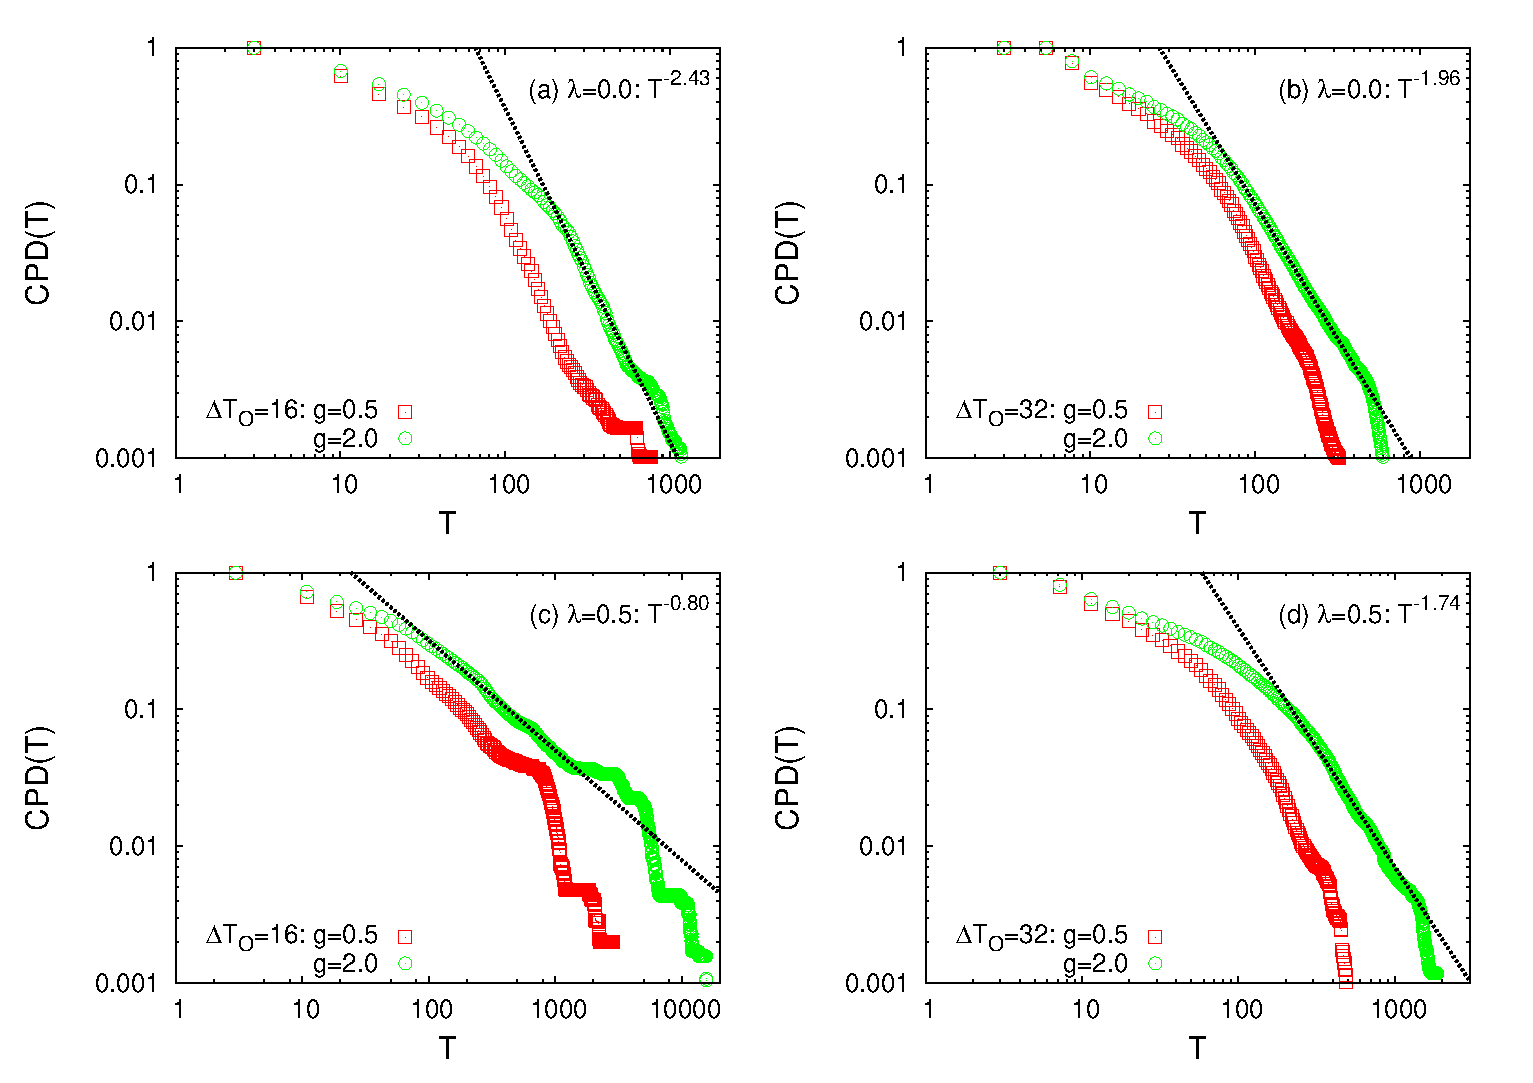
\includegraphics[width=12cm]{Ti.eps} 
\caption{Cumulative probability distribution of the travel times $\Delta t_{OD}$ in the $M=1.6\times 10^5$ trips. The lattice size is $L=40$ and $\alpha=0$ here.}\label{Ti}
\end{figure}


\begin{figure}
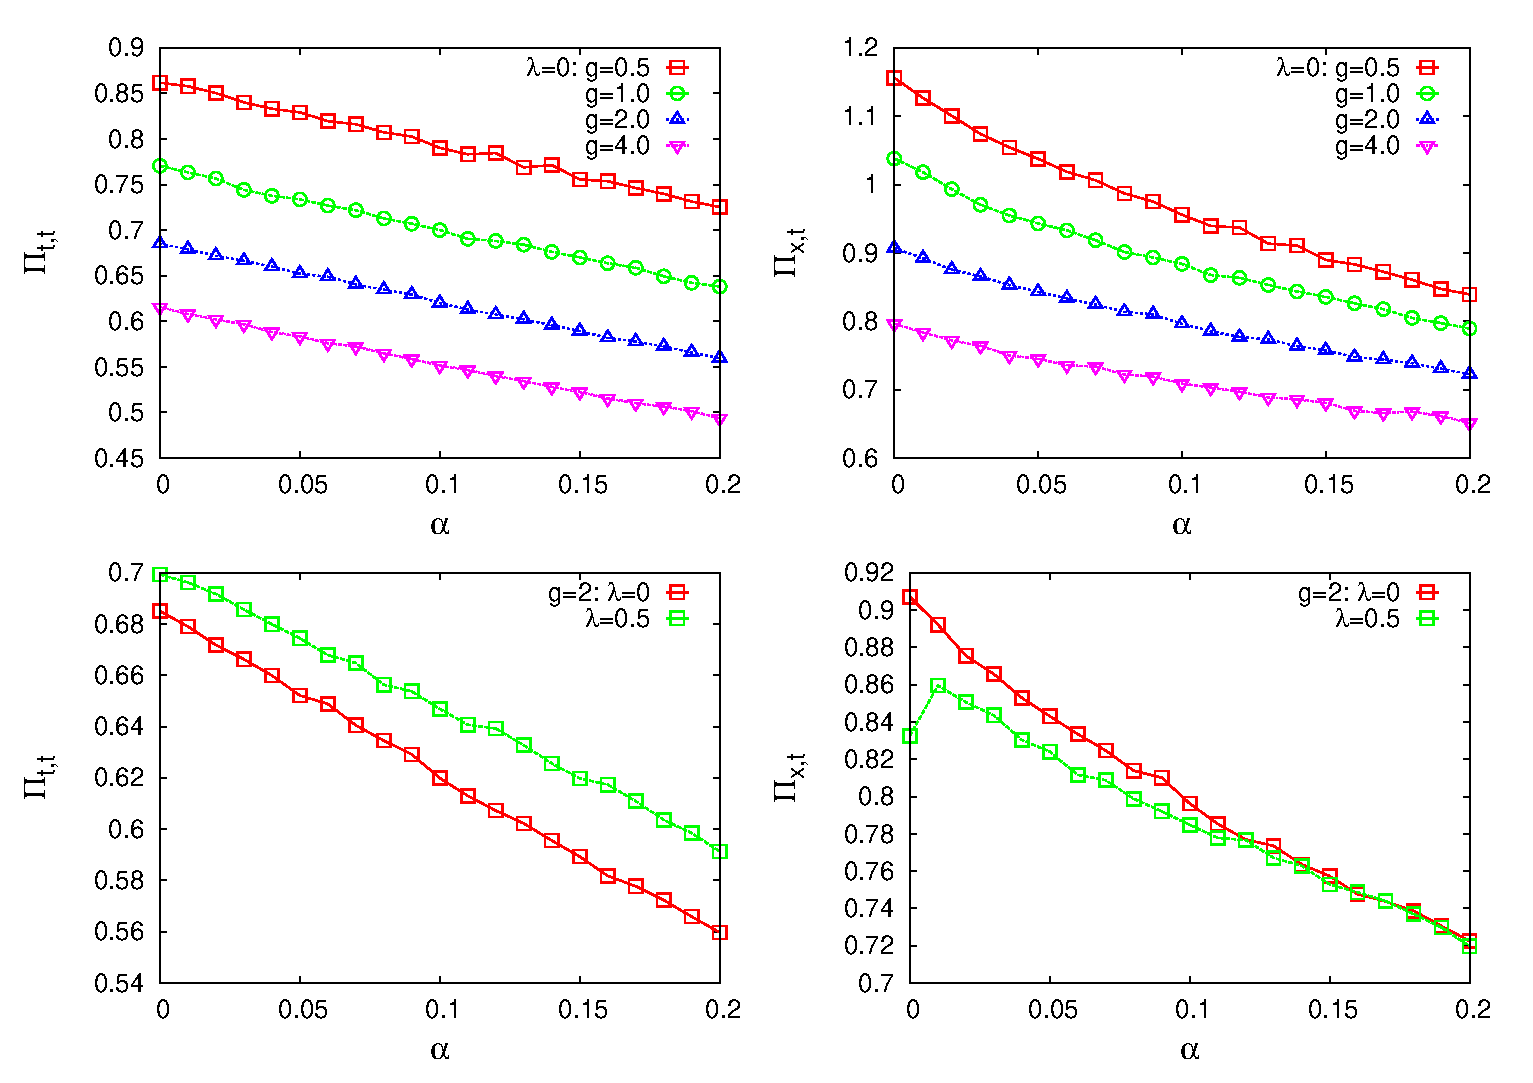
\includegraphics[width=12cm]{Pi.eps} 
\caption{Mutual information of origin times with destination times $\Pi_{t,t}$ and geometrical distances with travel times $\Pi_{x,t}$. The lattice size is $L=20$, and $\Delta T_O=16$ here. The data are averaged over $1000$ independnet realizations of the population distribution and the movement process.}\label{Pi}
\end{figure}


\begin{figure}
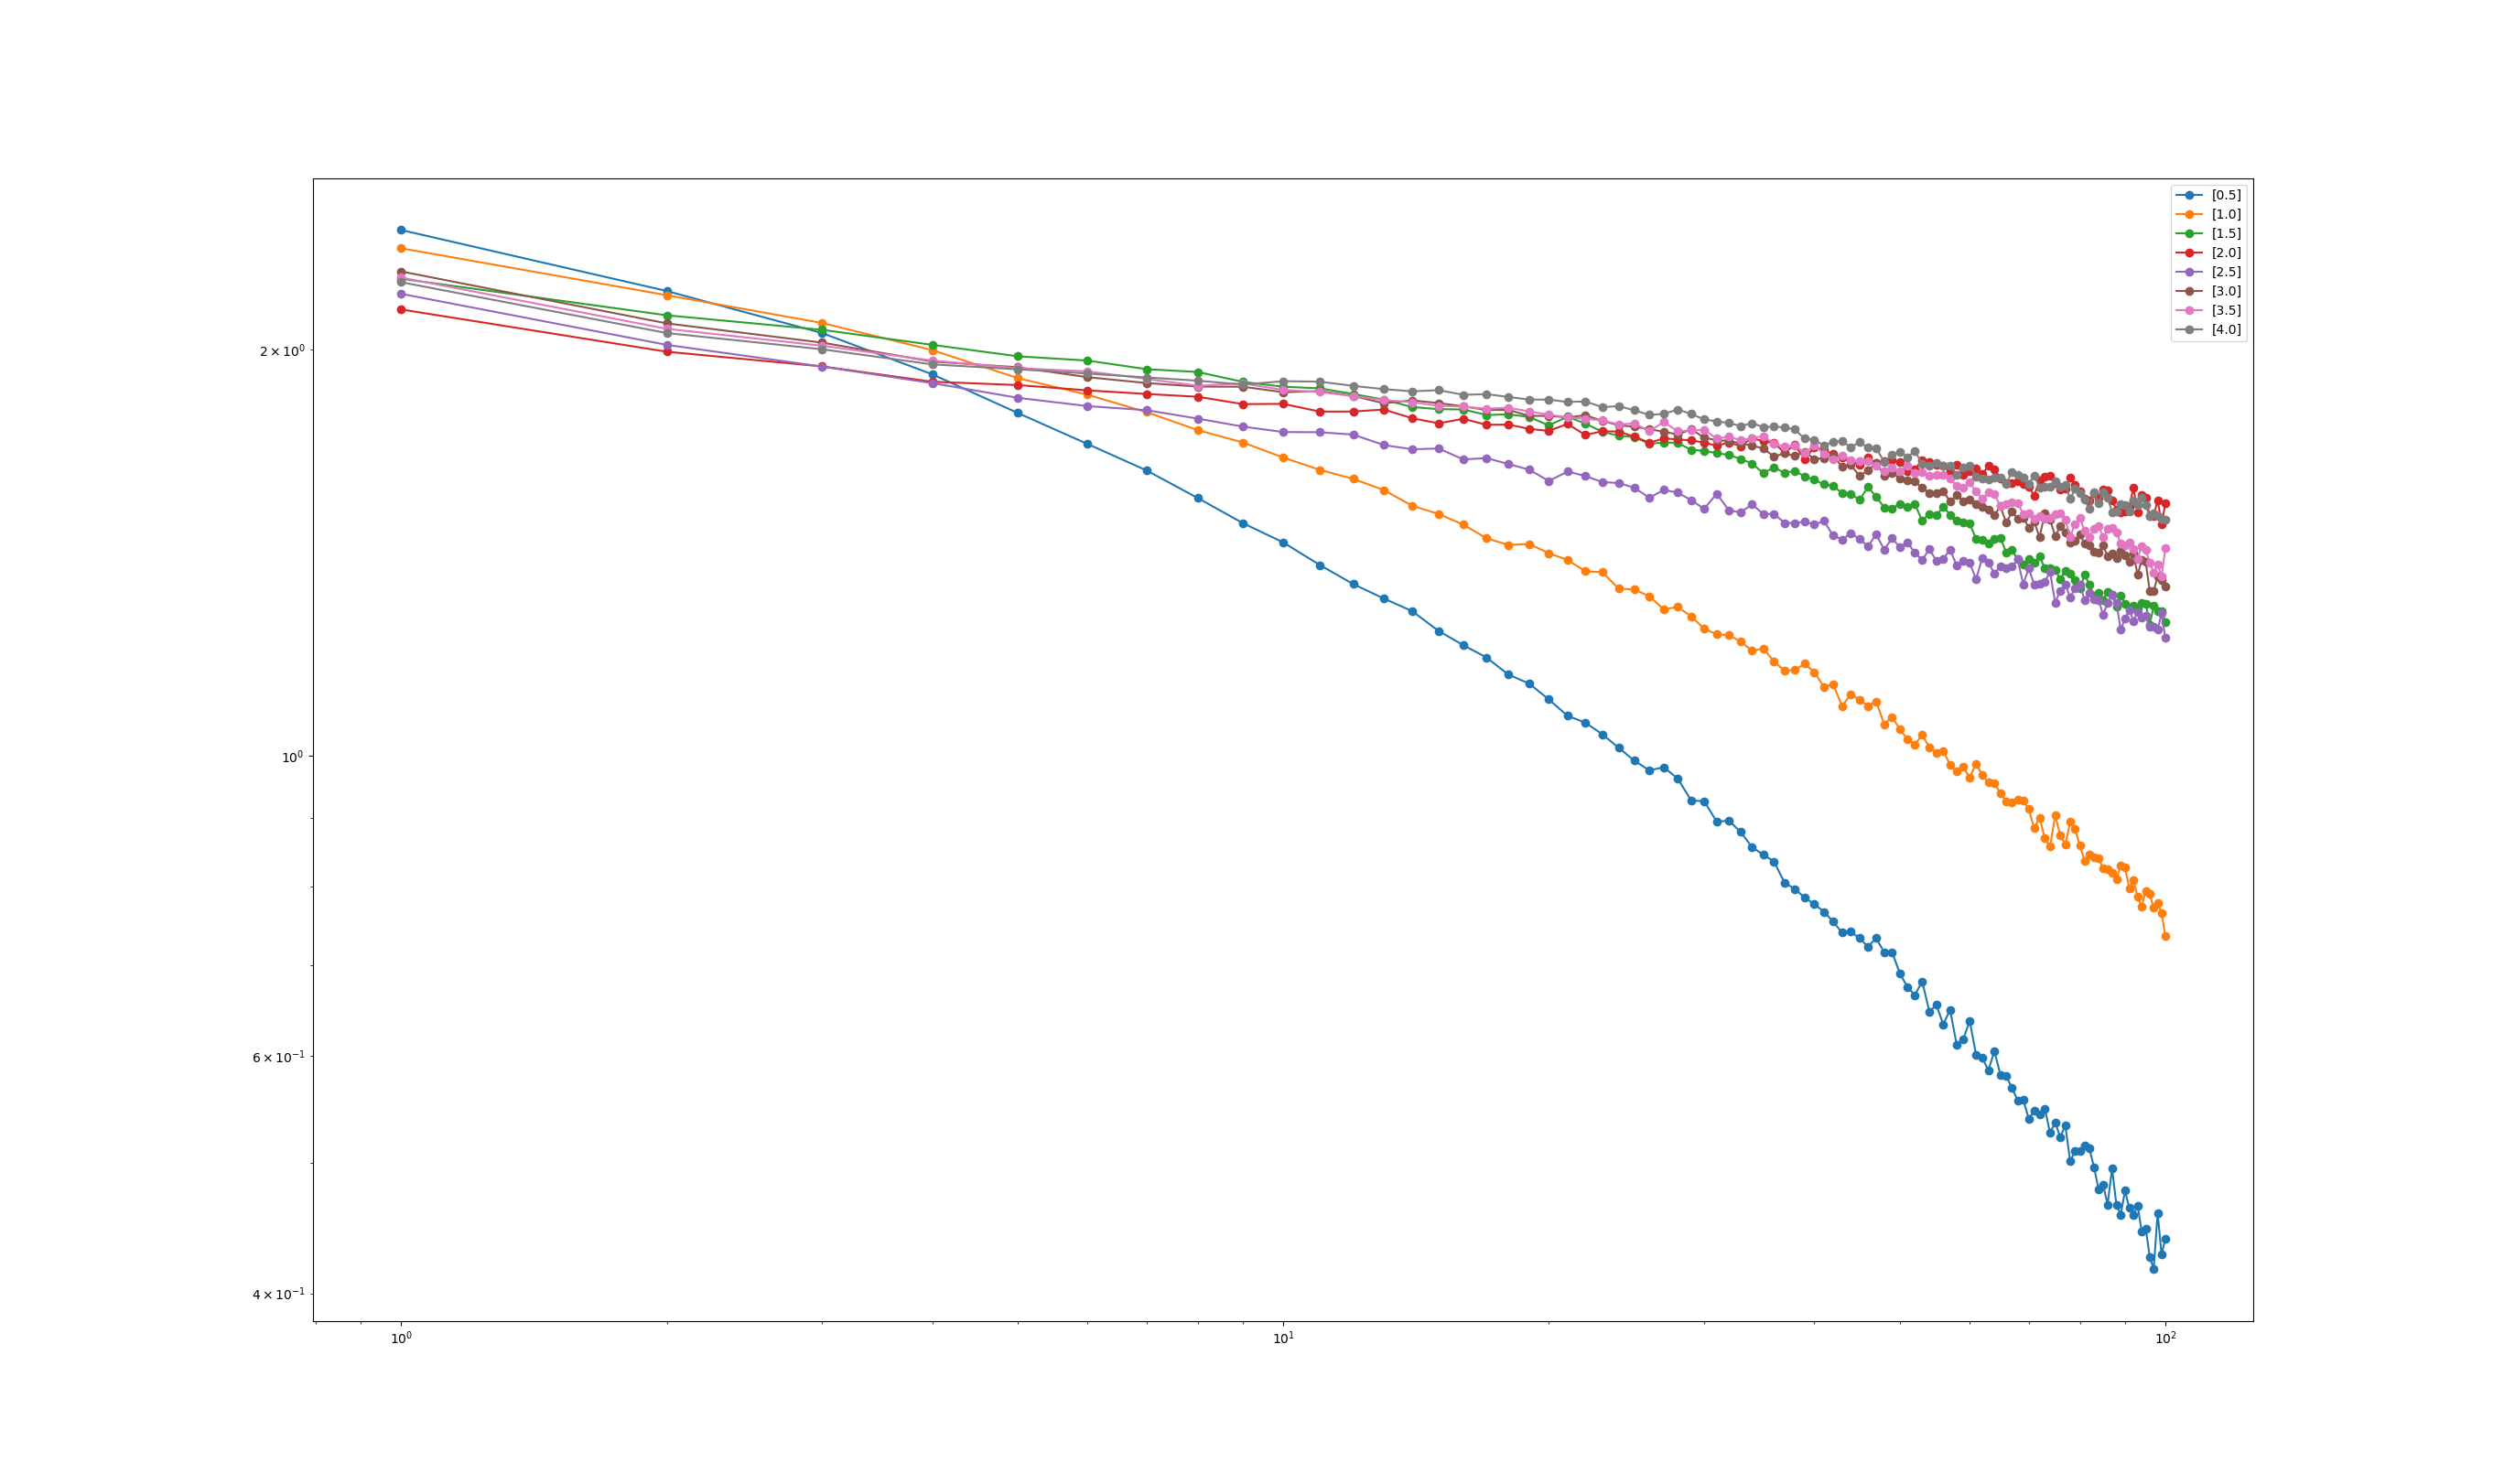
\includegraphics[width=12cm]{Rmax_loglog.png} 
\caption{Sample entropy vs the scale factor $w$. The lattice size is $L=20$, $\Delta T_O=16$, and $\alpha=0$ here. The data are for a single realization of the population distribution and the movement process.}\label{Sw}
\end{figure}


\begin{figure}
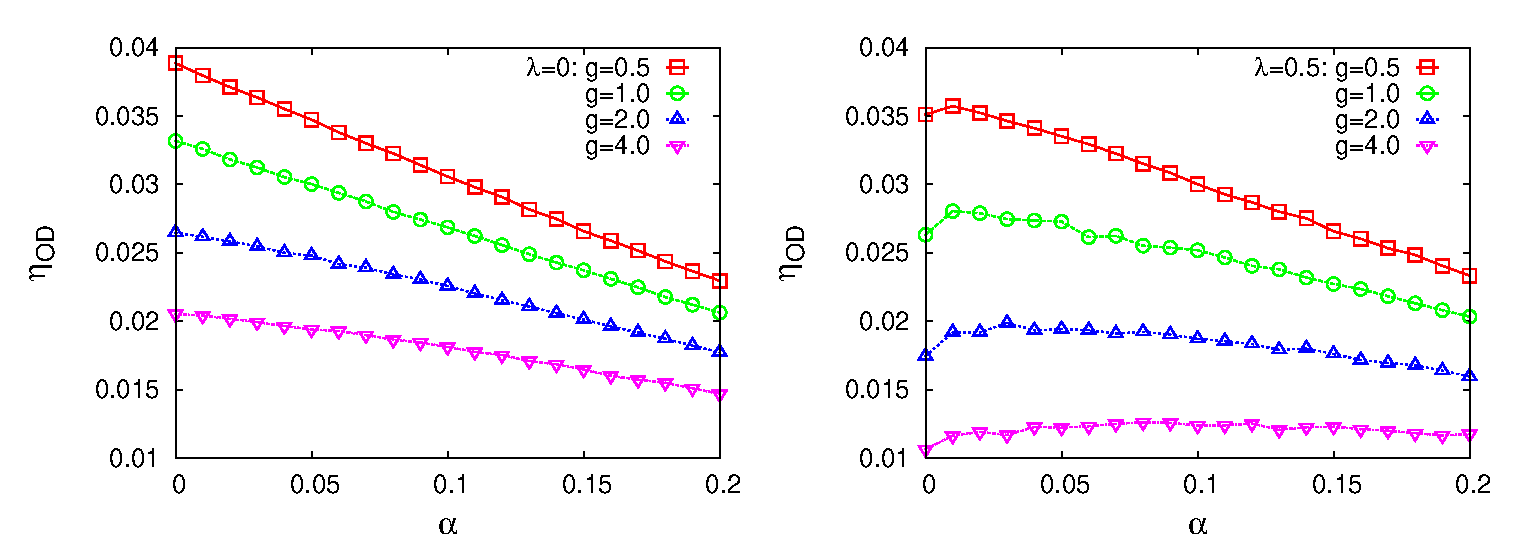
\includegraphics[width=12cm]{Ef.eps} 
\caption{The efficiency $\eta_{OD}$ vs the disorder parameter $\alpha$. The lattice size is $L=20$, and $\Delta T_O=16$ here. The data are averaged over $1000$ independnet realizations of the population distribution and the movement process. }\label{Ef}
\end{figure}


\begin{figure}
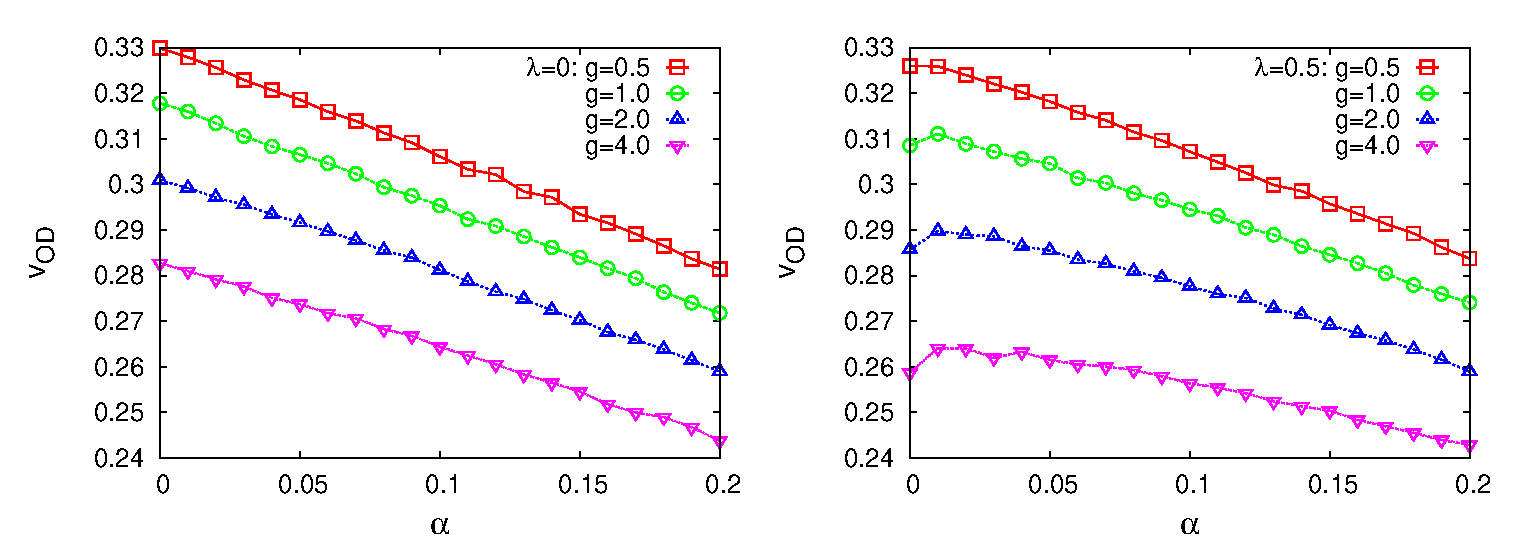
\includegraphics[width=12cm]{v.eps} 
\caption{The velocity $v_{OD}$ vs the disorder parameter $\alpha$. The lattice size is $L=20$, and $\Delta T_O=16$ here. The data are averaged over $1000$ independnet realizations of the population distribution and the movement process.}\label{v}
\end{figure}



\begin{figure}
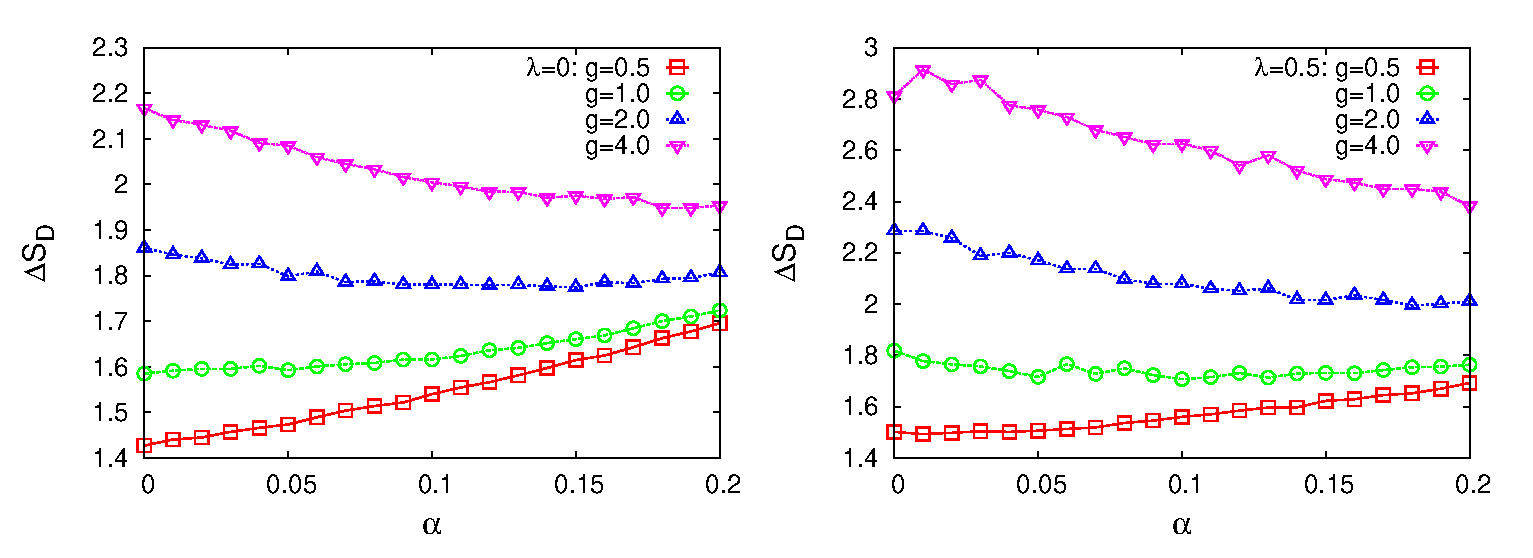
\includegraphics[width=12cm]{dS.eps} 
\caption{The relative entropy $\Delta S_D$ vs the disorder parameter $\alpha$. The lattice size is $L=20$, and $\Delta T_O=16$ here. The data are averaged over $1000$ independnet realizations of the population distribution and the movement process.}\label{dS}
\end{figure}



\begin{figure}
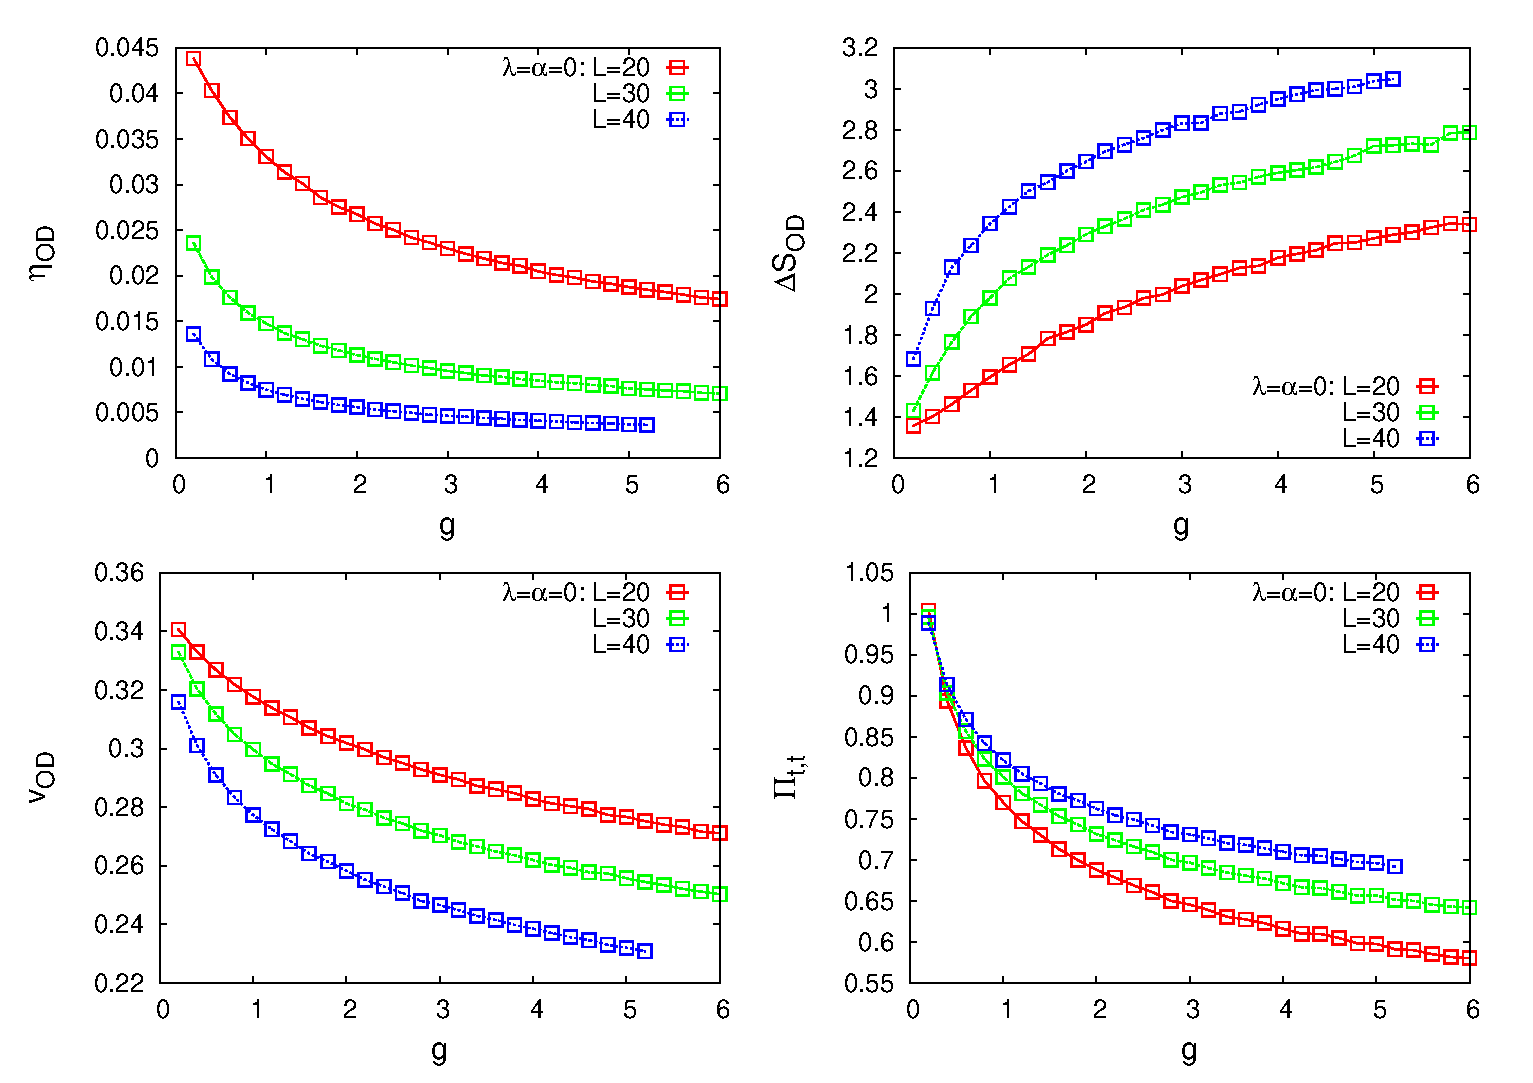
\includegraphics[width=12cm]{Lg.eps} 
\caption{Size effects with the interaction parameter $g$ for $\lambda=0$. Here $\Delta T_O=16, 24, 32$ for $L=20, 30, 40$, respectively to have the ratio $L/\Delta T_O$ fixed. Also the population density is fixed to $M/N=10^3$. The data are averaged over $1000$ (for $L=20,30$) or $500$ (for $L=40$) independnet realizations of the population distribution and the movement process.}\label{Lg}
\end{figure}


\begin{figure}
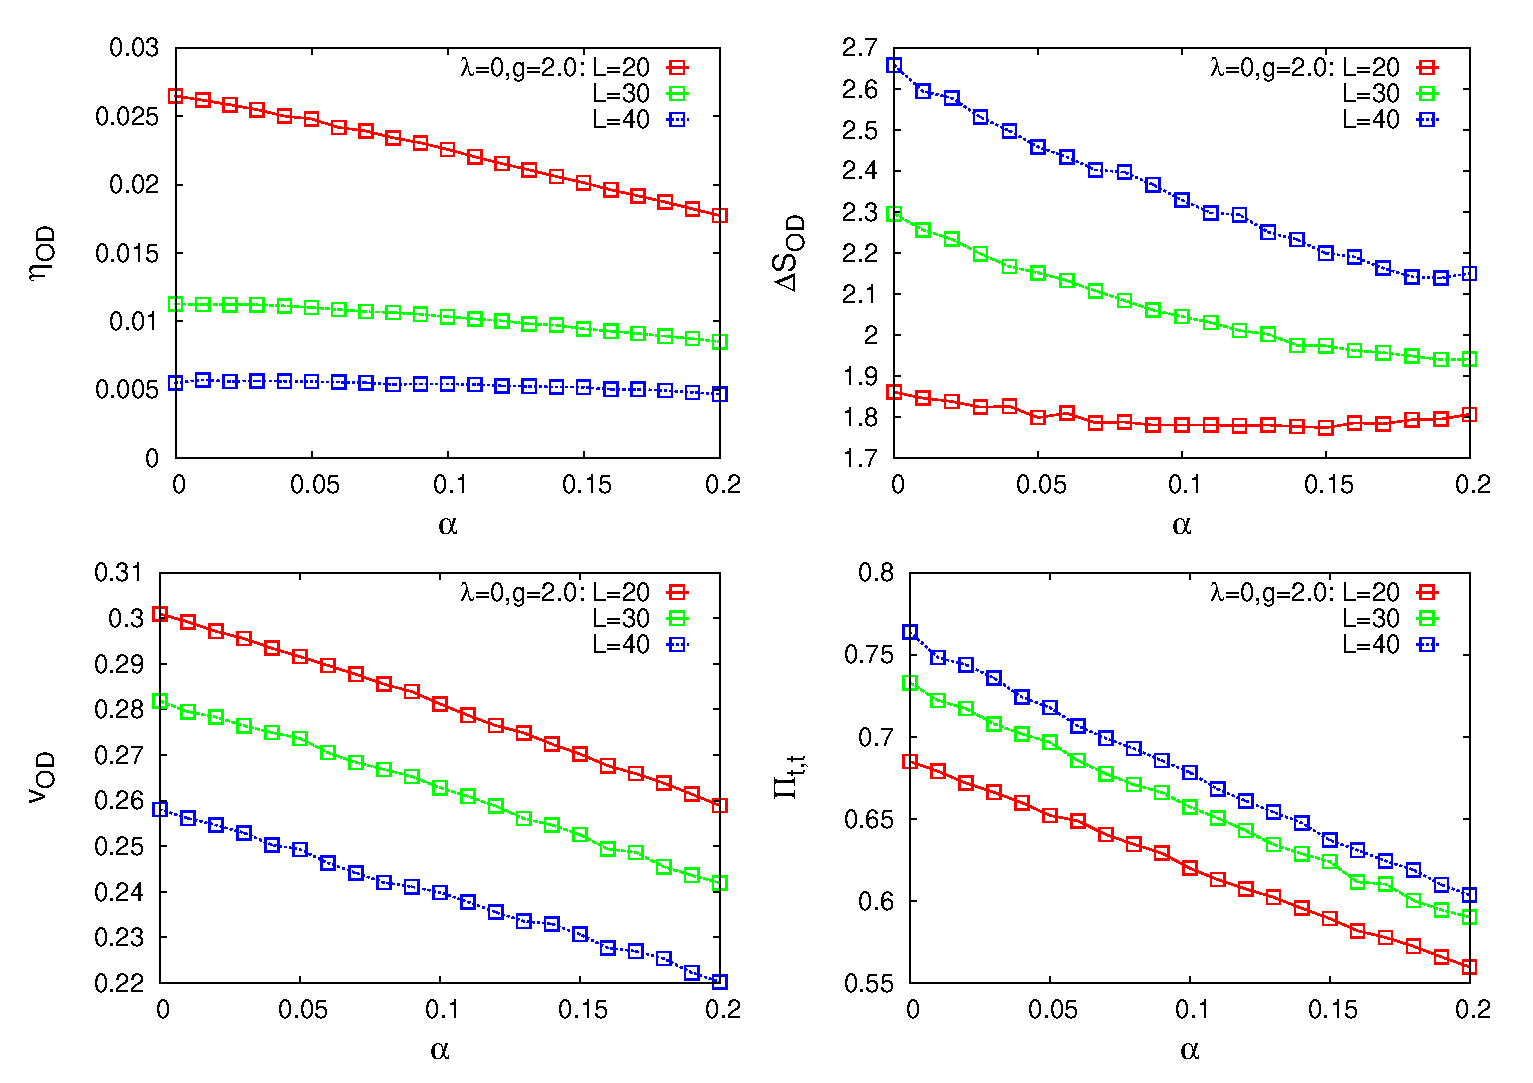
\includegraphics[width=12cm]{La.eps} 
\caption{Size effects with the disorder parameter $\alpha$ for $\lambda=0$. Here $\Delta T_O=16, 24, 32$ for $L=20, 30, 40$, respectively to have the ratio $L/\Delta T_O$ fixed. Also the population density is fixed to $M/N=10^3$. The data are averaged over $1000$ (for $L=20,30$) or $500$ (for $L=40$) independnet realizations of the population distribution and the movement process.}\label{La}
\end{figure}


\begin{figure}
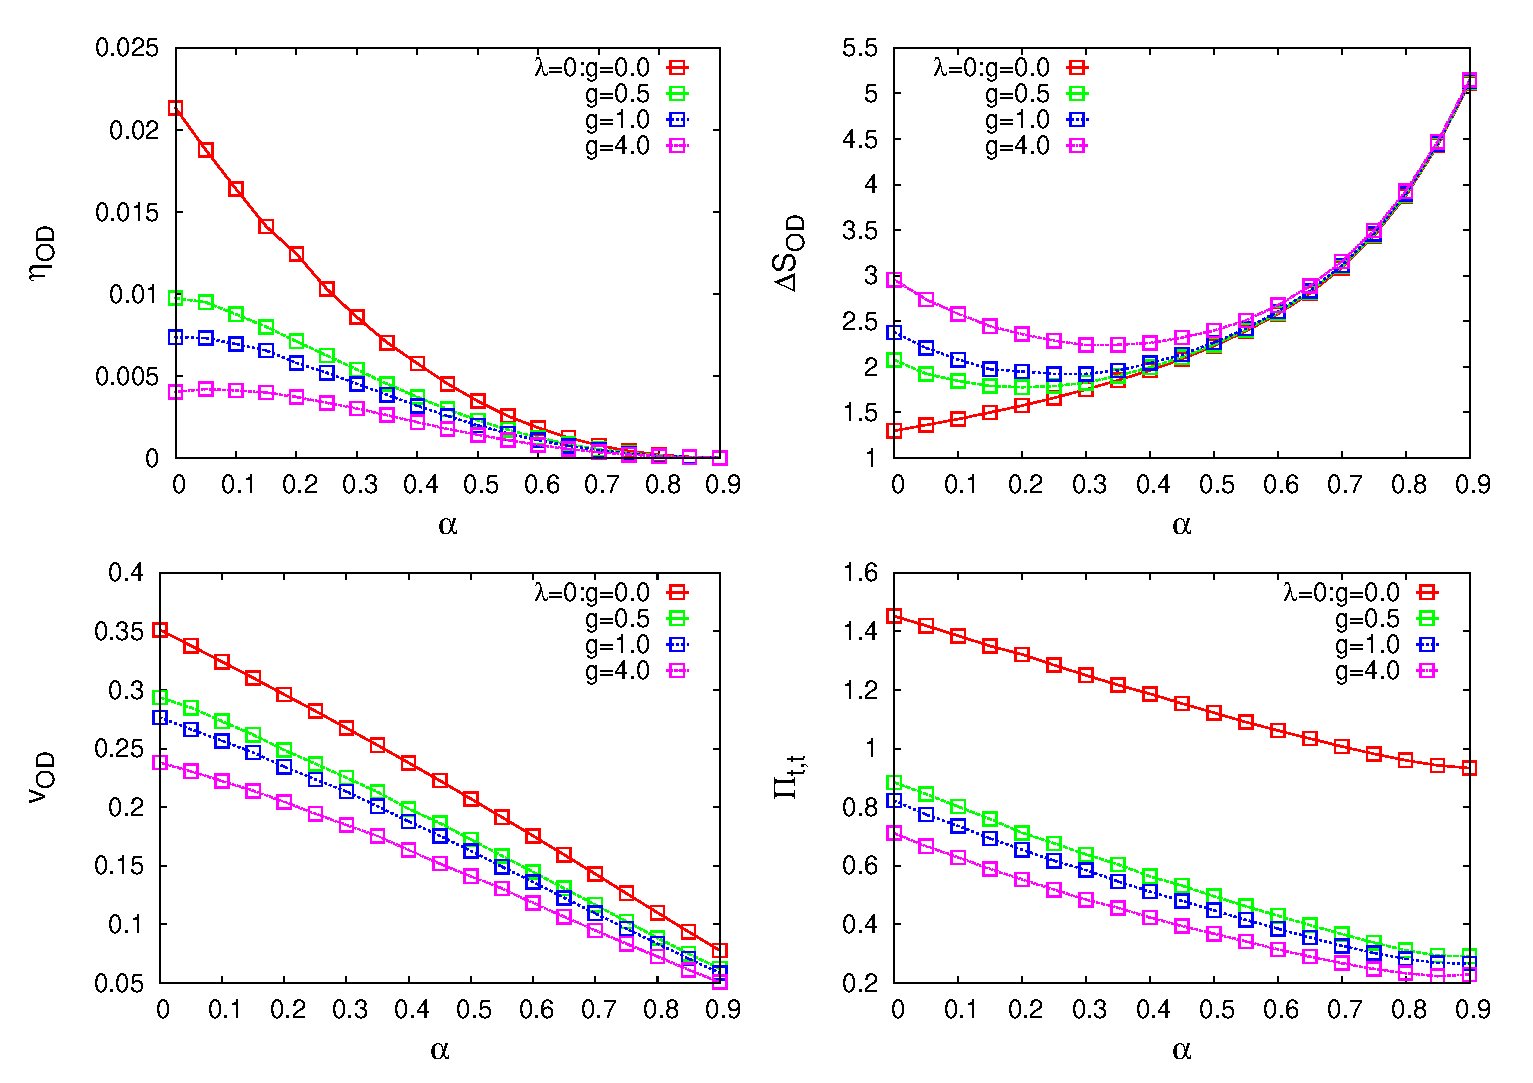
\includegraphics[width=12cm]{L4.eps} 
\caption{Behaviour in a larger range of the disorder parameter $\alpha$ for $\lambda=0$. The lattice size is $L=40$, and $\Delta T_O=32$ here. The data are averaged over $500$ independnet realizations of the population distribution and the movement process.}\label{L4}
\end{figure}




\end{document}


